\chapter{Analysis}

In this chapter I will shortly describe the dataset provided for this task, go over related work, then describe the frameworks and tools that are available. In the end I draw a conclusion and decide on how to proceed.

\section{Dataset}

The provided dataset consists of about 2'000 microscopic images with and without asbestos fibers. The images come in two different dimensions and different qualities. Most of the images are 1024 by 1024 pixels and using up 1.1 MB of disk space but some are in 1024 by 768 pixels and use only around 700 kB of disk space. The smaller images were originally in TIF format which needed to be converted into PNG format for better being able to load them into pyhton objects. All images are in grey color space. [TODO: why are there three channels then in python tensor???]. In figure \ref{fig:asbestos_examples} three images with a asbestos fiber are shown whereas in figure ... three images without asbestos are shown.

\begin{figure}[h]
\centering
\subfigure{
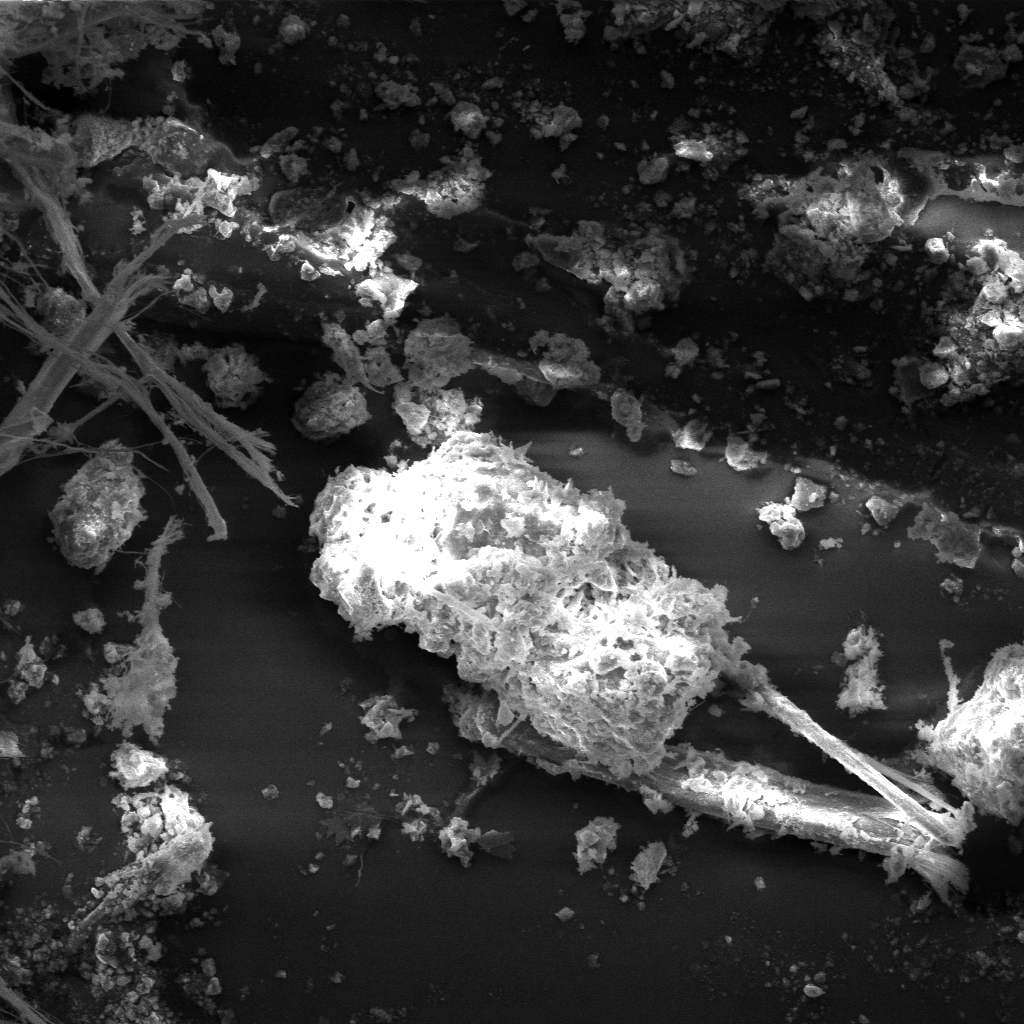
\includegraphics[width=.3\textwidth]{images/chapter2/asbestos_one.png}
}
\subfigure{
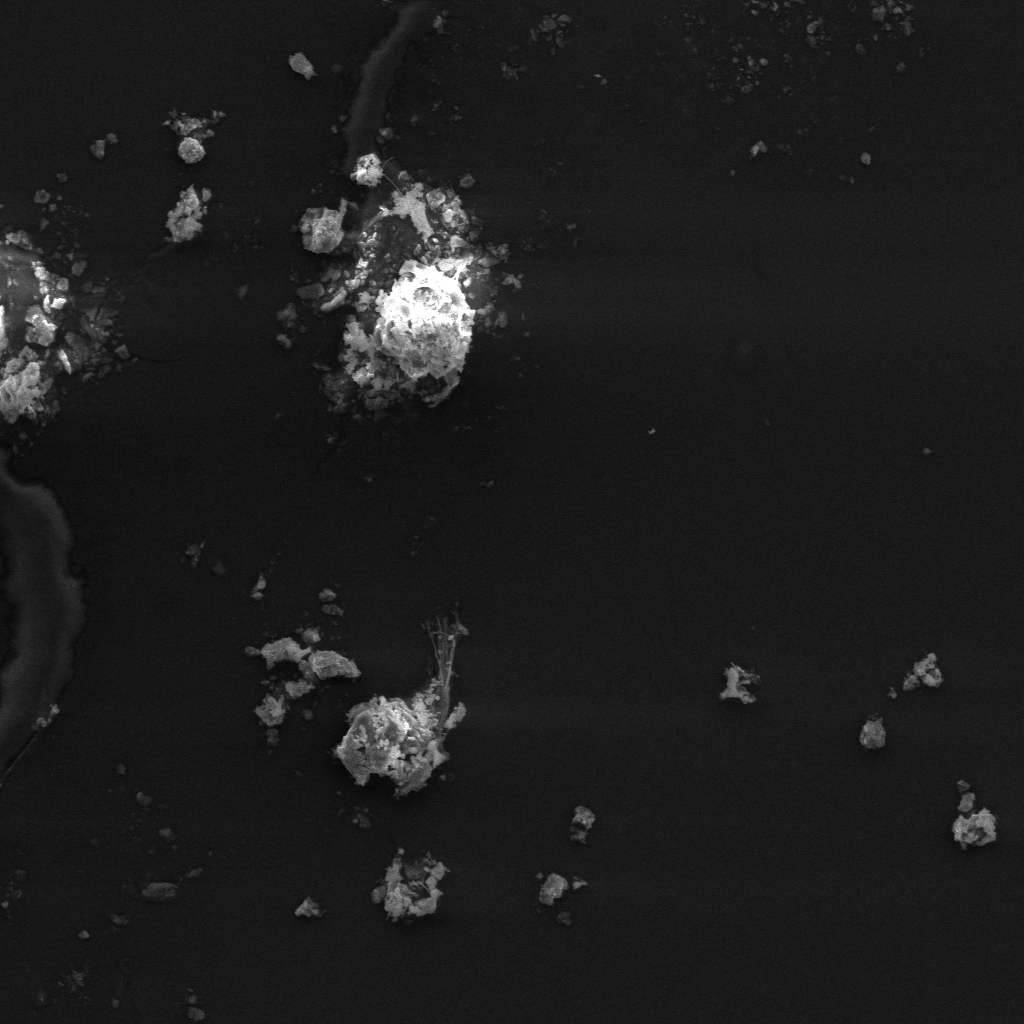
\includegraphics[width=.3\textwidth]{images/chapter2/asbestos_two.png}
}
\subfigure{
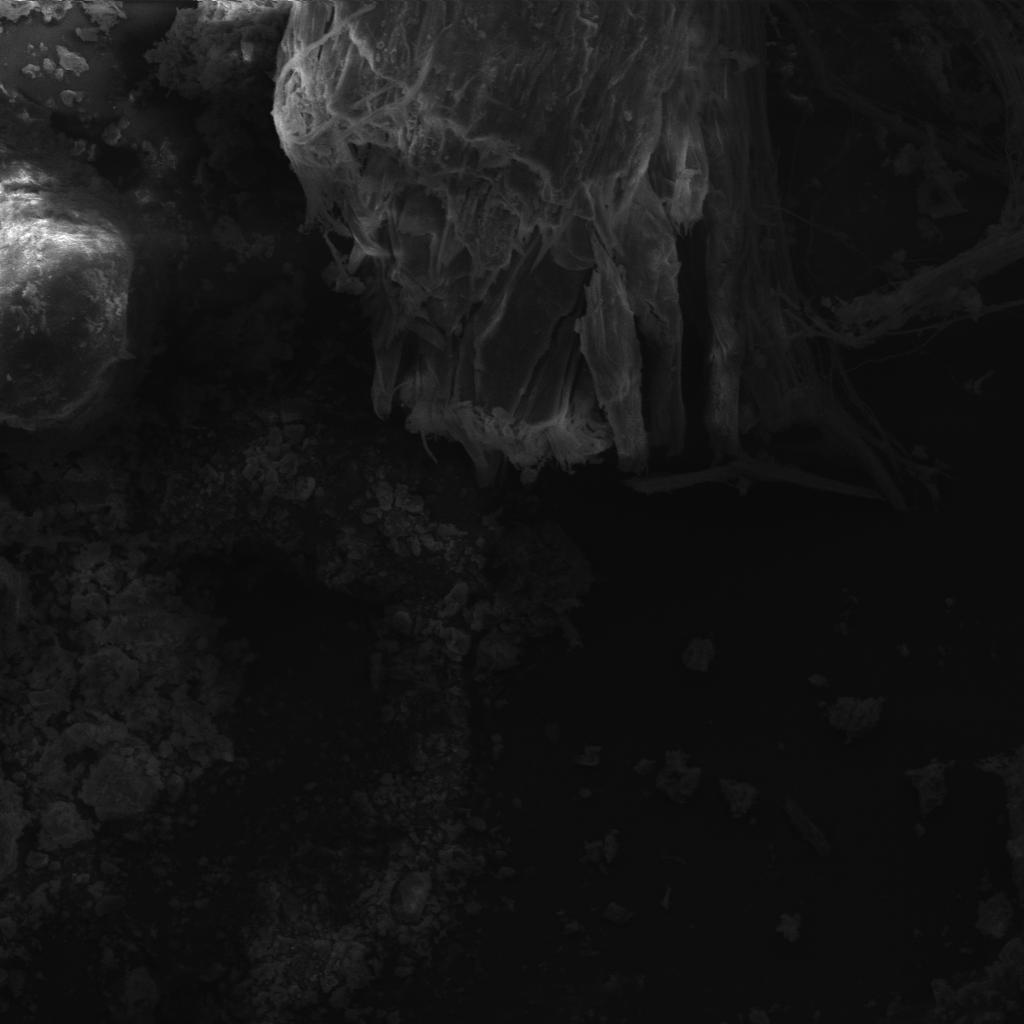
\includegraphics[width=.3\textwidth]{images/chapter2/asbestos_three.png}
}

\caption{Three examples of images with asbestos fibers. On the left the asbestos fibers are clearly visible, in the middle it's much harder to find them. In the right image there might be none, although the image is labelled as having asbestos in it.}
\label{fig:asbestos_examples}
\end{figure}

\begin{figure}[h]
\centering
\subfigure{
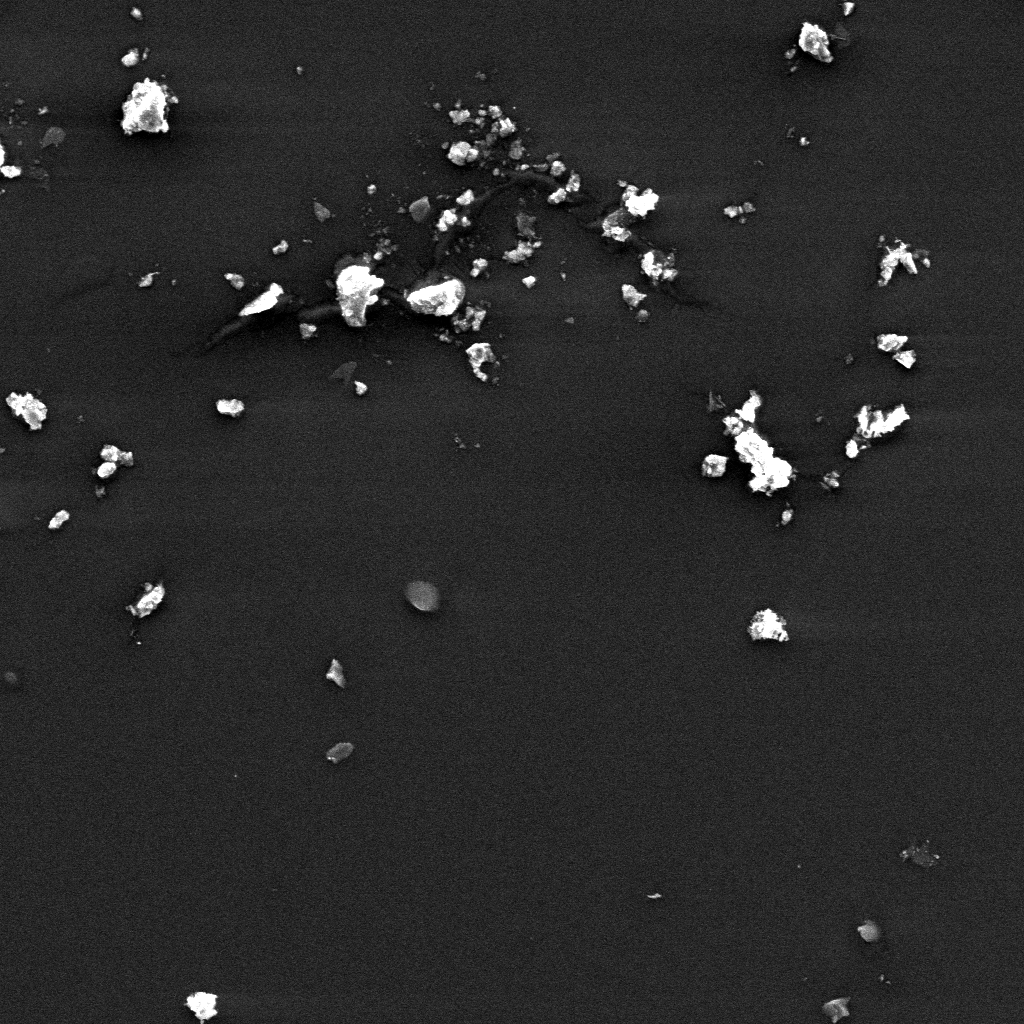
\includegraphics[width=.3\textwidth]{images/chapter2/non-asbestos_one.png}
}
\subfigure{
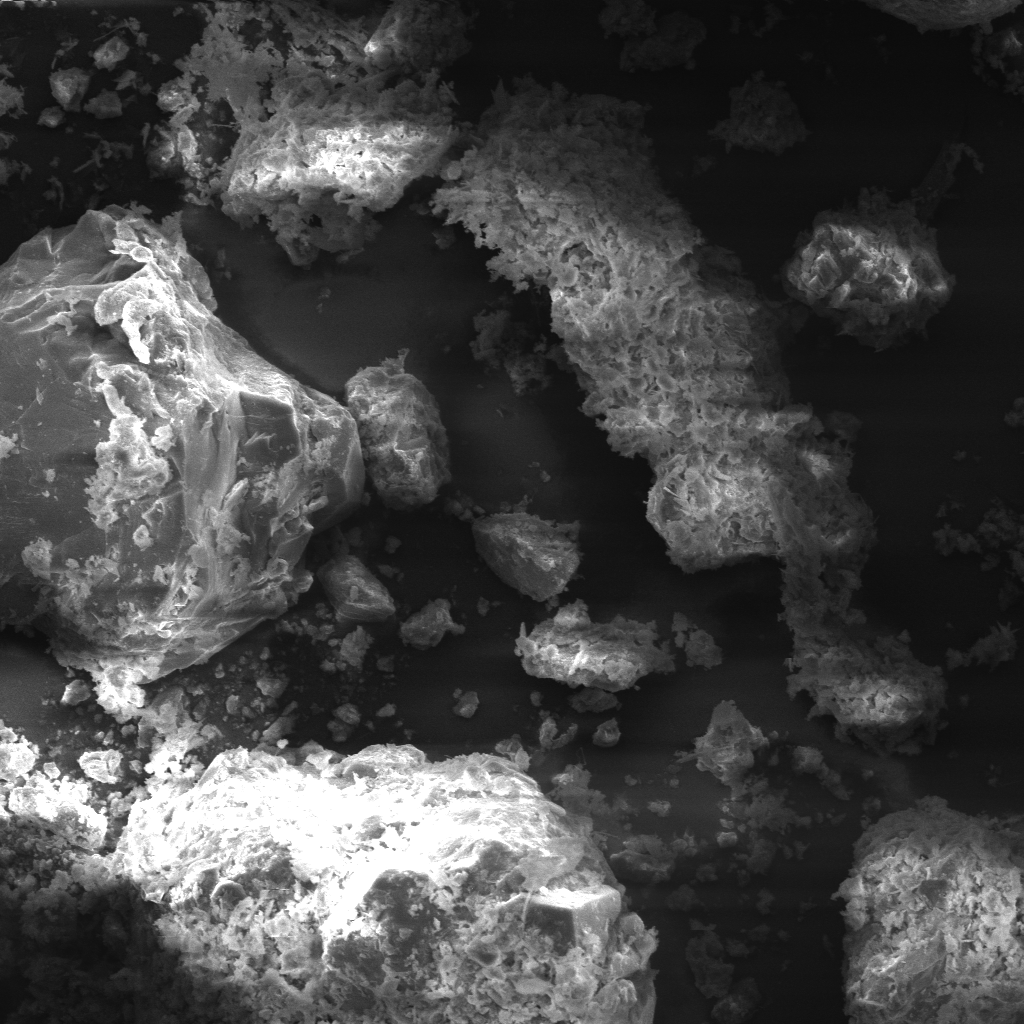
\includegraphics[width=.3\textwidth]{images/chapter2/non-asbestos_two.png}
}
\subfigure{
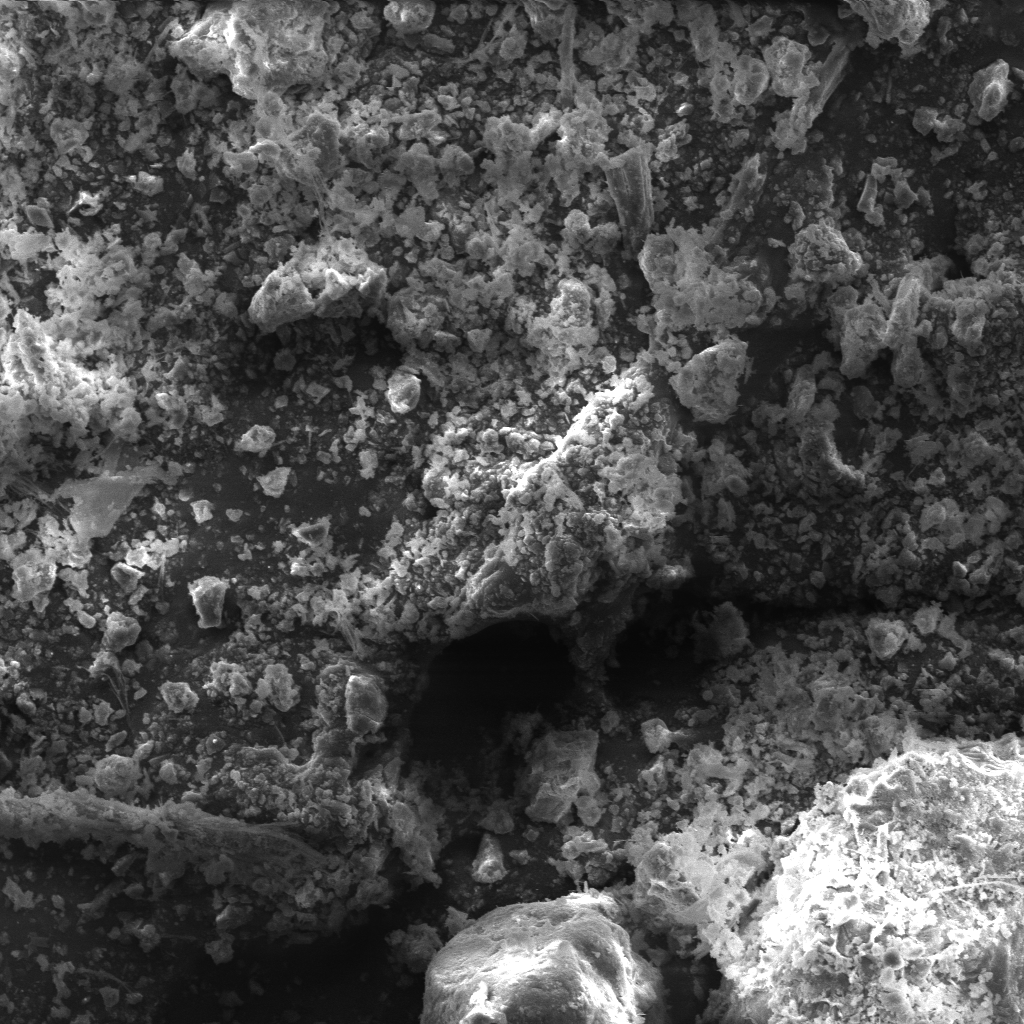
\includegraphics[width=.3\textwidth]{images/chapter2/non-asbestos_three.png}
}

\caption{Three examples of images without asbestos fibers. On the left image, there is clearly no asbestos to be found. In the middle and left image it's already much more difficult to be certain that there is none.}
\label{fig:non-asbestos_examples}
\end{figure}

As one difficult example (of many) I would like to show an image that was labeled and checked by the laboratory as having no asbestos in it. Nonetheless there are several areas where asbestos like structures emerge once the image is made brighter with an photo editing tool, especially a long fiber on the left side of the image marked by two arrows. This is to show, that the labeling will most certainly have errors in it, and that some images might look like having asbestos fibers in it but actually don't and the other way around. In order to be sure, the probes are examined chemically in a second phase that is not part of the masterthesis. Therefore it is more important to have less false positives than false negatives.

\begin{figure}[h]
\centering

\subfigure{
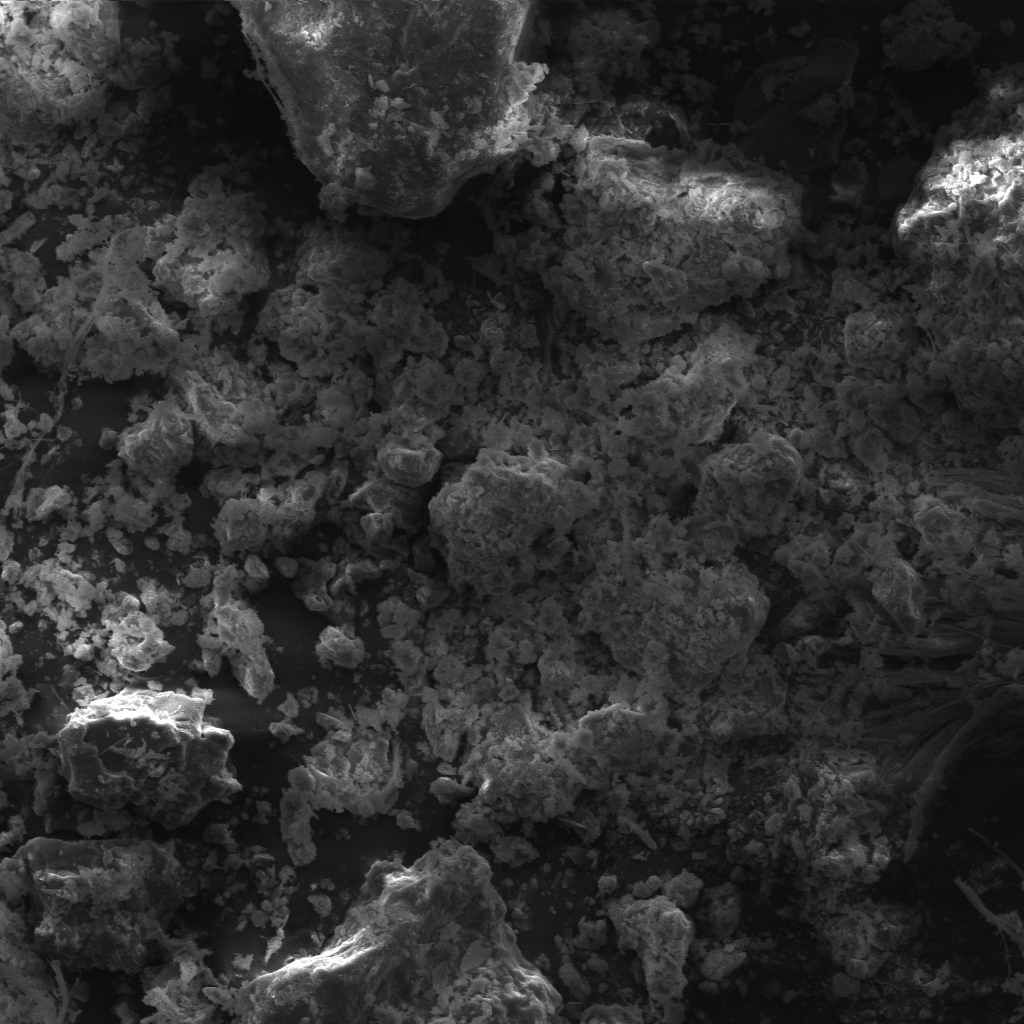
\includegraphics[width=.4\textwidth]{images/chapter2/probably_wrong_label.png}
}
\subfigure{
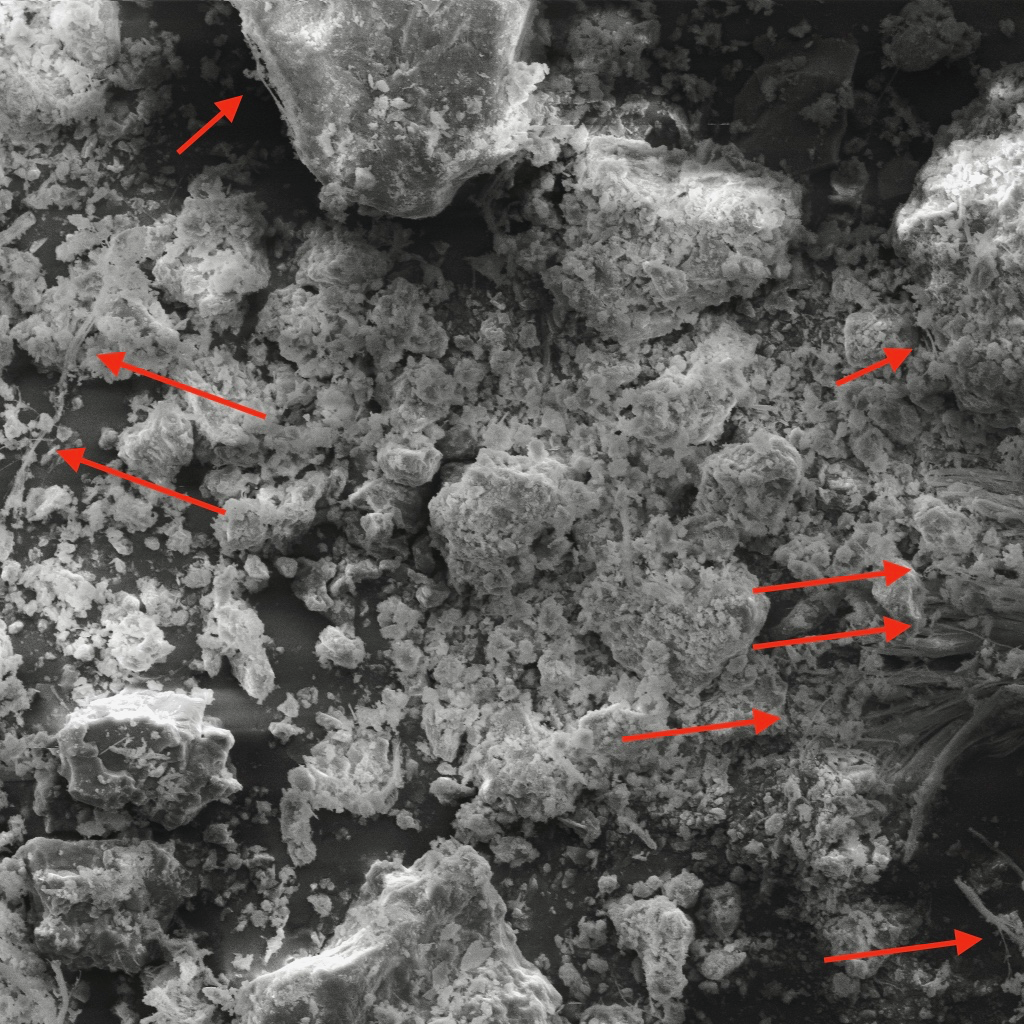
\includegraphics[width=.4\textwidth]{images/chapter2/probably_wrong_label_edited.png}
}

\caption{After brightening up the image and looking at it carefully, many different asbestos like structures emerge.}
\label{fig:non-asbestos_examples}
\end{figure}

\section{Related Work}

There are many different forms of asbestos that occur mostly in different materials and environments. Therefore the detection and quantification methods are quite different as well. In this chapter I will give a brief overview on related work on asbestos detection and focus on asbestos fiber detection from microscopic images with the help of statistical methods and deep learning. \\




Asbestos detection can be done in a variety of ways, [what ways + ref]

Asbestos can occur in many different forms and 

Looking for publications on Google Scholar for << asbestos detection method "microscope images" >>

\section{Deeplearning Frameworks}

There are two main Deeplearning Frameworks that can readily be used. Tensorflow \cite{tensorflow} which was originally developed by researchers and engineers at Google Brain and is based on Theano and PyTorch \cite{pytorch} that was built by researchers at Facebook. They are both open source and free to use, but the flavor is quite different. While TensorFlow uses static computational graphs that need to be built prior to compilation and run in their run engine, PyTorch uses dynamic computational graphs that can be more interpreted than compiled. Programming in PyTorch is much more pythonic whereas in TensorFlow the user needs first to get used to the Tensorflow way of doing things. Like building the whole computational graph in advance, using placeholders for all weights and variables, then creating a session in which the graph can be executed. Debugging in Tensorflow is more difficult since it needs at least two different debuggers to be used. One for the tensors and their values, and one for the python code itself. That makes it much less intuitive to simply debug the underlying code while keeping track of all tensors. In PyTorch the native debugger may be used for the whole codebase, including all the variables and weights. Data parallelisme is much easier to use in PyTorch since the distribution of the code and data onto all the GPU's happens automatically. Whereas in Tensorflow much more manual work and careful thought needs to be applied to achieve the same behaviour. Since PyTorch is one big framework it gives more the feeling of working with one framework that uses a very pythonic way to handle things. TensorFlow on the other hand is more like an aggregation of many libraries that work together to achieve a common goal. Although that was the case in early 2018 things are changing very fast for these frameworks. Tensorflow was much better for production environments but with PyTorch version 1.0 this advantage is closing fast \cite{pytorchOnePointZero}. Table \ref{tbl:DeepLearningFrameworks} summarizes the different qualities of  both frameworks at the start of the Masterthesis in late summer 2018. \\

\begin{table}[t] \centering
\ra{1.3}
\caption{Different qualities of the Deeplearning frameworks: PyTorch and Tensorflow)}
\begin{tabular}{@{}rrr@{}}
\toprule & PyTorch & TensorFlow \\
\midrule
Open-source									& + & + \\
Dynamic Computational Graph			& + & -  \\
Static Computational Graph				& - & +  \\
Easy Learning Curve							& + & -  \\
Fast developing of new Models			& + & -  \\
Production Environment					& - & + \\
Developer Community						& + & + \\
Native Visualization							& - & +  \\
Debugging										& + & -  \\
Data-Parallelisme								& + & -  \\
Framework-Feeling							& + & -  \\
Library-Aggregation							& - & +  \\

\bottomrule
\end{tabular}
\label{tbl:DeepLearningFrameworks}
\end{table}


There are some higher level frameworks like Keras \cite{keras} and DeepDIVA \cite{deepdiva} that enable many more things and faster development. Keras is build on top of TensorFlow and has many models pre-implemented. It enables the developer to very quickly start modeling a problem or apply already present architectures to new data. It does not allow the same flexibility as TensorFlow but if a new architectre needs to be designed from scratch it is done in TensorFlow, than made available on Keras as to use on different datasets or different tasks. A possible counterpart for Keras is DeepDIVA that was built on top of PyTorch and also provides pre-implemented architectures or allows to include them in a straigth-forward manner. It tackles some of the disadvantages of PyTorch versus Tensorflow like including TensorBoard Visualization to PyTorch. Development in DeepDIVA is also very pythonic and does not actually change at all since it is very tightly integrated in the PyTorch framework. Creating new architectures is or altering existing ones is straight forward.

\section{Tools}

Visualizing what the models learn is important to find logical errors and improve the architecture.

\section{Conclusion}

For me the most important thing was the ability to work in a very pythonic way and be able to start developing my models quickly without having to learn new frameworks. Debugging is one of the most crucial things when learning how to code new problems and because of these two main reasons my choice fell towards PyTorch. Additionally, I decided to go with DeepDIVA on top of PyTorch. It gives me many of the advantages that applied previously only to tensorflow like simple visualization of the results and learning process through tensorboard, but it also gives me some very useful pre-implemented architectures to start from. \\

For the visualization of the different layers of the network I decided to go with Utku Ozbulak's visualization toolbox \cite{viztoolbox}. It is implemented in PyTorch and can be easily applied with some tweakings to the current models. It has many different visualization modes to chose from and is quite extensive. It also provides a heat maps for easy localization of the object.